\section{Ajuste de modelo de masa}

\subsection{Marco teórico}

Se quiere encontrar una fórmula analítica para la curva de rotación basándose en un modelo físico que considere la distribución de masa de la galaxia.

Se iguala para cierta partícula de masa $m$ en rotación pura la fuerza de gravedad con la fuerza centrípeta,
\begin{equation}
G\frac{M(R)m}{R^2}=m\frac{v_\textnormal{rot}^2(R)}{R}
,\end{equation}
donde $G$ es la constante de gravitación universal y $M$ es la masa de la galaxia dentro de un radio $R$ determinado por la distancia galactocéntrica de la partícula. Luego, la velocidad de rotación de la curva de rotación de la figura \ref{eq:vrot} se puede modelar por,
\begin{equation}
v_\textnormal{rot}(R)=\sqrt{G\frac{M(R)}{R}}
.\label{eq:vmass}\end{equation}

Se estudian cinco modelos de distribución de masa para la galaxia, listados a continuación.
\begin{itemize}
\item Masa puntual en el centro de la galaxia. $M(R)=M_0$. $M_0$ es el parámetro libre de la masa puntual.

\item Disco uniforme. $M(R)=\pi R^2s_0$. $s_0$ es el parámetro libre de densidad superficial uniforme de masa.

\item Esfera uniforme. $M(R)=\frac{4}{3}\pi R^3\rho_0$. $\rho_0$ es el parámetro libre de densidad uniforme volumétrica de masa.

\item Disco uniforme con una masa puntual en el centro. $M(R)=\pi R^2s_0+M_0$. Dos parámetros libres, $s_0$ y $M_0$.

\item Esfera uniforme con una masa puntual en el centro. $M(R)=\frac{4}{3}\pi R^3\rho_0+M_0$. Dos parámetros libres, $rho_0$ y $M_0$.
\end{itemize}

\subsection{Detalla del algoritmo}

El código X muestra el sigueinte procedimiento. Se evalúan los cinco modelos de distribución de masa en la ecuación \ref{eq:vmass} y se realiza un ajuste no lineal de mínimos cuadrados según el algoritmo de Levenberg-Marquardt para cada modelo, asumiendo una desviación estándar de la unidad para las velocidades de rotación. Además, se calcula el error RMS de cada modelo con respecto a las velocidades de rotación medidas para determinar el mejor ajuste.

\subsection{Ajuste de los modelos de la curva de rotación}

La tabla \ref{tab:massmodel} muestra el resultado del ajuste de mínimos cuadrados con los parámetros óptimos para cada modelo de distribución de masa de la Galaxia y el error RMS con respecto a la velocidad rotacional medida.

La figura \ref{fig:massmodel} muestra el gráfico de los ajustes de los cinco modelos de distribución de masa de la Galaxia.

\begin{table*}[htpb]
	\centering
	\begin{tabular}{lcccc}
		\toprule
		{Modelo} &
		{$M_0$} &
		{$s_0$} &
		{$\rho_0$} &
		{RMS} \\
		{} &
		{$\textnormal{M}_\odot$} &
		{$\textnormal{M}_\odot\,\textnormal{kpc}^{-2}$} &
		{$\textnormal{M}_\odot\,\textnormal{kpc}^{-3}$} &
		{\si{\kilo\meter\per\second}} \\
		\midrule
		Punto & $3.655\times10^{10}\pm1.321\times10^{9}$ & --- & --- & $68.738$ \\
		Disco & --- & $6.419\times10^{8}\pm5.501\times10^{6}$ & --- & $17.248$ \\
		Esfera & --- & --- & $8.569\times10^{7}\pm1.883\times10^6$ & $43.337$ \\
		Disco + Punto & $3.928\times10^{9}\pm3.422\times10^{8}$ & $5.814\times10^{8}\pm6.851\times10^{6}$ & --- & $14.749$ \\
		Esfera + Punto & $1.259\times10^{10}\pm4.343\times10^{8}$ & --- & $6.127\times10^{7}\pm1.112\times10^{6}$ & $21.326$ \\
		\bottomrule
	\end{tabular}
	\caption{Parámetros y error obtenido del ajuste no lineal de míminos cuadrados para los modelos de distribución de masa de la Galaxia con respecto a la velocidad rotacional medida.}\label{tab:massmodel}
\end{table*}

\begin{figure}[htbp]
	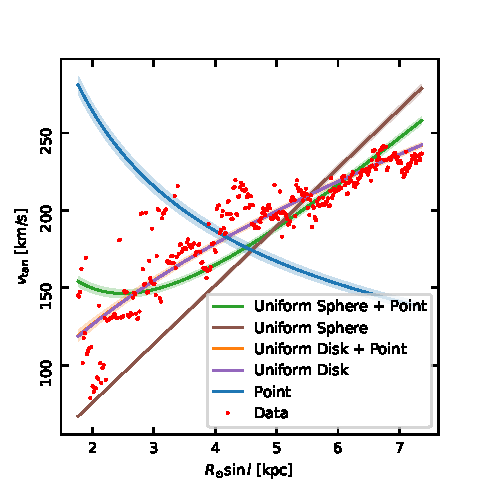
\includegraphics{rsc/massmodels.pdf}
	\caption{Ajuste de los modelos de distribución de masa de la Galaxia con respecto a la curva de rotación medida. Línea negra es datos medidos. Línea naranja es modelo de masa puntual central. Línea verde es modelo de disco uniforme. Línea naranja es modelo de esfera uniforme. Línea azul es modelo de disco uniforme con masa puntual central. Línea morada es modelo de esfera uniforme con masa puntual central. Las cinco líneas de ajustes tienen un área respectiva que representa el error de los parámetros óptimos.}
	\label{fig:massmodel}
\end{figure}
